% !TeX root = chapter-6-7-8.tex

\selectlanguage{hebrew}

%\begin{comment}

\chapter{חשבון דיפרנציאלי ואינטגרלי}


%%%%%%%%%%%%%%%%%%%%%%%%%%%%%%%%%%%%%%%%%%%%%%%%%%%%%%%%%%%%%%%%%%%%%%

\section{קיץ תשע"ז מועד ב}

\begin{center}
\selectlanguage{english}
\includegraphics[width=\textwidth]{summer-2017b-8}
\end{center}

\vspace{-2ex}

\textbf{סעיף א}

הערך של 
$f(x)$
שלילי בין
$0$
ל-%
$\frac{\pi}{2}$,
ולכן:
\[
S_1+S_2=\int_0^{\frac{\pi}{2}} -f(x) dx + \int_\frac{\pi}{2}^{2\pi} f(x) dx = 10\pi^2+16\,.
\]
נתון ש:
\[
-S_1+S_2=\int_0^{\frac{\pi}{2}} f(x) dx + \int_\frac{\pi}{2}^{2\pi} f(x) dx=\int_0^{2\pi} f(x) dx =8\pi^2\,.
\]
יש לנו שתי משוואות עבור שני הנעלמים
$S_1,S_2$
והפתרון הוא:
\[
S_1=\pi^2+8\,.
\]

\textbf{סעיף ב}

\[
-S_1=\int_0^{\frac{\pi}{2}} f(x) dx = \left. F\right|_0^{\frac{\pi}{2}}=F\left(\frac{\pi}{2}\right)- F(0)=F\left(\frac{\pi}{2}\right)=-(\pi^2+8)\,.
\]

\np

\textbf{סעיף ג}

נתון ש-%
$f\left(\disfrac{\pi}{2}\right)=0$.
\erh{12pt}
\begin{equationarray*}{rcl}
f(x) &=& \int f'(x) dx= \int (8\sin x + 8) dx\\
&=&-8\cos x + 8x + c\\
f\left(\disfrac{\pi}{2}\right) &=& -8\cos \frac{\pi}{2} + 8\cdot \frac{\pi}{2} + c = 0\\
c&=&-4\pi\\
f(x) &=& -8\cos x + 8x -4\pi\,.
\end{equationarray*}

\np

%%%%%%%%%%%%%%%%%%%%%%%%%%%%%%%%%%%%%%%%%%%%%%%%%%%%%%%%%%%%%%%%%%%%%%

\section{קיץ תשע"ז מועד ב}

\begin{center}
\selectlanguage{english}
\includegraphics[width=\textwidth]{summer-2017a-8}
\end{center}

\vspace{-2ex}

\textbf{סעיף א}

נציב את הביטויים הנתונים עבור 
$A,B$
ונקבל שתי משוואת בשני נעלמים
$t,c$
שנוכל לפתור:
\erh{2pt}
\begin{equationarray*}{rcl}
-(2t)^2+2(2t)+c&=&0\\
-(-t)^2+2(-t)+c&=&0\\
-3t^2+6t&=&0\\
t(6t-3)&=&0\\
t&=&2\\
-(-2)^2+2(-2)+c&=&0\\
c&=&8\,.
\end{equationarray*}
פסלנו את הפתרון
$t=0$
כי נתון ש-%
$t>0$.

הפונקציה היא
$f(x)=-x^2+2x+8$.

\textbf{סעיף ב}

נקודת החיתוך על ציר הסימטריה של הפרבולה היא נקודת המקסימום של
$f(x)$.
מהנגזרת הראשונה
$f'(x)=-2x+2=0$
מתקבל
$x=1$.

$ML$
הוא בסיס המשולש ו-%
$KL$
הוא הגובה. חישוב השטח ונקודת האיפוס של הנגזרת הוא:
\erh{10pt}
\begin{equationarray*}{rcl}
S(x)&=&\frac{1}{2}(x-1)(-x^2+2x+8)\\
S'(x)&=&\frac{1}{2}\cdot -3x^2+6x+6=0\\
x&=&\frac{2\pm\sqrt{4-4\cdot 2}}{2}=1\pm\sqrt{3}\,.
\end{equationarray*}

השטחים הם מקסימליים כי חישוב הנגזרת השנייה נותן:
\erh{2pt}
\begin{equationarray*}{rcl}
S''(x)&=&-6x+6\\
S''(1+\sqrt{3})&=&-\sqrt{3}<0\,.
\end{equationarray*}

הפתרון
$1+\sqrt{3}$
מתאים למשולש בתרשים. הפתרון
$1-\sqrt{3}$
מתאים למשולש הסימטרי משמאל ל-%
$M$.
אורך הבסיס יהיה
$1-x$
והסימנים יתהפכו ונקבל שטח חיובי ומקסימלי.

\begin{quote}
פתרונות אחרים משתמשים במונח "קודקוד הפרבולה". לא נתקלתי בו בספרי לימוד או בבחינות אחרות. עבור פרבולה
$ax^2+bx+c$
ערך ה-%
$x$
של הקודקוד הוא
$\frac{-b}{2a}$.
לדעתי אין צורך לזכור את הנוסחה כי ניתן לשחזור אותה על ידי חישוב הנגזרת:
\erh{2pt}
\begin{equationarray*}{rcl}
f(x)&=&ax^2+bx+c\\
f'(x)&=&2ax+b=0\\
x&=&\frac{-b}{2a}\,.
\end{equationarray*}
\end{quote}

\np


%%%%%%%%%%%%%%%%%%%%%%%%%%%%%%%%%%%%%%%%%%%%%%%%%%%%%%%%%%%%%%%%%%%%%%

\section{קיץ תשע"ה מועד ב}

\begin{center}
\selectlanguage{english}
\includegraphics[width=\textwidth]{summer-2015b-8a}
\includegraphics[width=\textwidth]{summer-2015b-8b}

\end{center}

\vspace{-2ex}

\textbf{סעיף א}

)בשאלה אין נוסחה לפנוקציה, גם לא לאחר פתרון השאלה, ולכן התרשים הוא ממש "סקיצה".(

\begin{center}
\selectlanguage{english}
\begin{tikzpicture}%[scale=.8]
\begin{axis}[
    axis lines=center,
    xmin = 0,
    xmax = 7,
    ymin = -4,
    ymax = 3.2,
    ymajorticks=false,
]
\addplot [
    smooth,
] plot coordinates
{(.1,-4) (.2,-3) (.4,-1.8) (.6,-1) (1,0) (2,2) (3,3) (4,2) (5,1) (6,0.5) (7,0.2)};
\fill (axis cs:1,0) circle(1.5pt);
\fill (axis cs:3,3) circle(1.5pt);
\end{axis}
\end{tikzpicture}
\end{center}

\textbf{סעיף ב}

קיימת נקודת קיצון ב-%
$x=1$
כי הנגזרת הראשונה מתאפסת. הנגזרת עולה ולכן מדובר במינימום.


\textbf{סעיף ג}

הנגזרת השנייה היא השיפוע של הנגזרת הראשונה, שהוא חיובי עבור
$0<x<3$
ושלילי עבור
$3<x$.
לכן הפונקציה קעורה כלפי מעלה ב-%
$0<x<3$
וקעורה כלפי מטה ב-%
$3<x$.


\textbf{סעיף ד}

אם הפונקציה מקבלת ערכים 
$y\geq 4$
אזי נקודות המינימום שמתקבלת ב-%
$x=1$
צריך לקבל את הערך
$y=4$.

נשתמש בנתון שלפונקציה יש 
\asm{}
ב-%
$x=0$,
וכיווני הקעירות מסעיף ג כדי להשלים את צורת הגרף:

\begin{center}
\selectlanguage{english}
\begin{tikzpicture}%[scale=.8]
\begin{axis}[
    axis lines=center,
    xmin = 0,
    xmax = 7.2,
    ymin = 0,
    ymax = 7.2,
]
\addplot [
    smooth,
] plot coordinates
{(.1,7) (.4,5) (.6,4.5) (1,4) (2,5.2) (3,6) (7,6.3)};
\fill (axis cs:1,4) circle(1.5pt);
\fill (axis cs:3,6) circle(1.5pt);
\end{axis}
\end{tikzpicture}
\end{center}


\textbf{סעיף ה}

$f(x)$
חיובית בכל תחום ההגדרה, לכן גם
$f^3(x)$
חיובית. סימן המינוס הופך את הסימן של ערך הפונקציה. 
$f(x)$
יורד ב-%
$0<x<1$
ולכן 
$g(x)$
עולה בתחום זה.
$f(x)$
עולה ב-%
$1<x$
ולכן 
$g(x)$
יורד בתחום זה.

בפתרונות אחרים לשאלה משתמשים בנגזרת של
$g(x)$:
\[
g'(x)=-3 f^2(x) f'(x)\,.
\]
$f^2(x)$
תמיד חיובי, ולכן לאור המינוס בתחילת הביטוי, תחומי העלייה והירדה הם התחומים שערכי
$f'(x)$
שליליים או חיוביים בהתאמה.
$f'(x)$
חותך את ציר ה-%
$x$
משליליים לחיוביים ב-%
$x=1$,
ולכן 
$g(x)$
עולה ב-%
$0<x<1$
ועולה ב-%
$1<x$.


\np


%%%%%%%%%%%%%%%%%%%%%%%%%%%%%%%%%%%%%%%%%%%%%%%%%%%%%%%%%%%%%%%%%%%%%%

\section{קיץ תשע"ה מועד א}

\begin{center}
\selectlanguage{english}
\includegraphics[width=\textwidth]{summer-2015a-8}
\end{center}

\vspace{-2ex}

\textbf{סעיף א}

נגזרת ראשונה:

\vspace{-5ex}

\erh{10pt}
\begin{equationarray*}{rcl}
f'(x)&=& x^2 -a^2=0\\
x&=&\pm a\\
f(+a)&=& -\frac{2}{3}a^3+a^2\\
f(-a)&=& \frac{2}{3}a^3+a^2\\
f''(x)&=&2x\\
f''(+a)&=&2a>0\\
f''(-a)&=&-2a<0\,.
\end{equationarray*}

\vspace{-4ex}

בשתי השורות האחרונות השתמשנו בנתון
$a>0$.
המקסימום הוא ב-%
$x=-a$.
שוב נשתמש בנתון 
$a>0$
ונקבל
$f(-a)=\frac{2}{3}a^3+a^2>0$.

\textbf{סעיף ב}

המינימום הוא ב-%
$x=a$.
נתון 
$a>0$
ולכן
$a^2$
לא משפיע על החישובים:
\erh{10pt}
\begin{equationarray*}{rcl}
f(a) &=& -\frac{2}{3}a^3+a^2 = a^2\left(-\frac{2}{3}a+1\right) = 0, \quad a=\frac{3}{2}%
\quad\quad\quad$x-$\textrm{\R{על ציר ה}}\\
f(a) &=& -\frac{2}{3}a^3+a^2 =a^2\left(-\frac{2}{3}a+1\right) > 0, \quad a<\frac{3}{2}%
\quad\quad\quad$x-$\textrm{\R{מעל ציר ה}}\\
f(a) &=& -\frac{2}{3}a^3+a^2 =a^2\left(-\frac{2}{3}a+1\right) < 0, \quad a>\frac{3}{2}%
\quad\quad\quad$x-$\textrm{\R{מתחת לציר ה}}\,.
\end{equationarray*}

\np

\textbf{סעיף ג}

נקודות המינימום מסומנות.

קו רציף: על הציר. קו מקווקוו: מעל לציר. קו מנוקד: מתחת לציר.

\begin{center}
\selectlanguage{english}
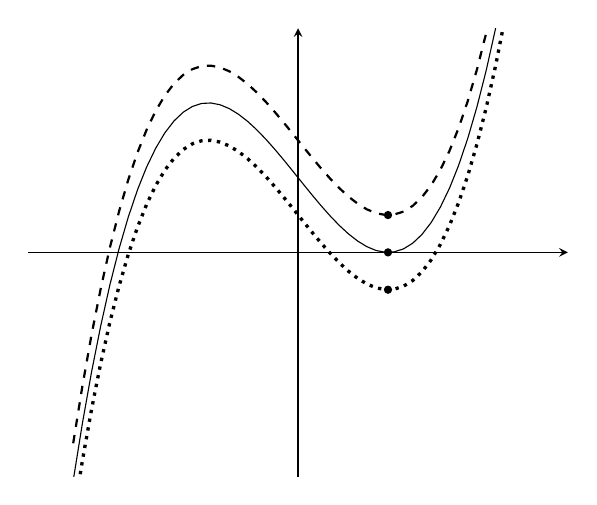
\begin{tikzpicture}%[scale=.8]
\begin{axis}[
    axis lines=center,
    xmin = -3,
    xmax = 3,
    ymin = -2,
    ymax = 2,
    xmajorticks=false,
    ymajorticks=false,
]
\addplot [
    domain=-2.5:2.5,
    samples=50,
]
{.333*x^3-x+1-.333};
\addplot [
    domain=-2.5:2.5,
    samples=50, 
    thick, dashed,
]
{.333*x^3-x+1};
\addplot [
    domain=-2.5:2.5,
    samples=50, 
    very thick, dotted,
]
{.333*x^3-x+1-.666};
\fill (axis cs:1,.333) circle(1.5pt);
\fill (axis cs:1,0) circle(1.5pt);
\fill (axis cs:1,-.333) circle(1.5pt);
\end{axis}
\end{tikzpicture}
\end{center}


\textbf{סעיף ד}

משוואה זו היא המשוואה הנתונה בשאלה כאשר
$a=1$.
אבל 
$1<\frac{3}{2}$,
ולכן לפי סעיף ב המינימום נמצא מעל לציר ה-%
$x$.
מכאן שאין פתרון אחר פרט לנקודת החיתוך של הגרף לפני המקסימום.

\np


%%%%%%%%%%%%%%%%%%%%%%%%%%%%%%%%%%%%%%%%%%%%%%%%%%%%%%%%%%%%%%%%%%%%%%

\section{חורף תשע"ה}

\begin{center}
\selectlanguage{english}
\includegraphics[width=\textwidth]{winter-2015-8}
\end{center}

\vspace{-2ex}

\textbf{סעיף א}

לפי הנוסחה לנגזרת של חזקה של פונקציה,
$(f(x)^{\frac{1}{2}})' = \frac{1}{2}f(x)^{-\frac{1}{2}}f'(x)$
שהיא הפונקציה המופיעה באינטגרל. נחשב את ערך האינטגרל:

\vspace{-3ex}

\erh{12pt}
\begin{equationarray*}{rcl}
\int_0^3 \frac{f'(x)}{2\sqrt{f(x)}} dx &=& \left. \sqrt{f(x)}\right|_0^3\\
&=&\sqrt{f(3)}-\sqrt{f(0)} = \sqrt{f(3)}-1=3\\
f(3)&=&4^2=16\,.
\end{equationarray*}

\vspace{-3ex}

הפונקציה
$f(x)$
מתקבלת מאינטגרציה של הנוסחה הנתונה לנגזרת ומחישוב הקבוע והפרמטר מהערכים הידועים של
$f(0),f(3)$:
\erh{12pt}
\begin{equationarray*}{rcl}
f(x)&=&\int (kx+2)dx = \frac{1}{2}kx^2+2x+c\\
f(0)&=&c=1\\
f(3)&=&\frac{9}{2}k+7=16\\
k&=&2\\
f(x)&=&x^2+2x+1\,.
\end{equationarray*}

\np


\textbf{סעיף ב}

\[
g(x)=\sqrt{f(x)}=\sqrt{(x+1)^2}\,.
\]
אם
$x\geq -1$,
$x+1$
לא שלילי ו-%
$g(x)=x+1$.

אם 
$x<-1$,
$x+1$
שלילי ו-%
$g(x)=-(x+1)$.

ביחד יש לנו
$g(x)=|x+1|$.


\medskip

\textbf{סעיף ג}

\begin{center}
\selectlanguage{english}
\begin{tikzpicture}%[scale=.8]
\begin{axis}[
    axis lines=center,
    xmin = -3,
    xmax = 3,
    ymin = -1,
    ymax = 2,
]
\addplot [
    domain=-3:2,
    samples=50,
]
{x^2+2*x+1};
\addplot [
    domain=-3:2,
    samples=50,
]
{abs(x+1)};
\fill (axis cs:0,1) circle(1.5pt);
\fill (axis cs:-1,0) circle(1.5pt);
\node at (axis cs: 1,1.5) {$g(x)$};
\node at (axis cs: -1.75,1.5) {$f(x)$};
\end{axis}
\end{tikzpicture}
\end{center}


\np

%%%%%%%%%%%%%%%%%%%%%%%%%%%%%%%%%%%%%%%%%%%%%%%%%%%%%%%%%%%%%%%%%%%%%%

\section{קיץ תשע"ד מועד ב}

\begin{center}
\selectlanguage{english}
\includegraphics[width=\textwidth]{summer-2014b-8}
\end{center}

\vspace{-2ex}

\begin{center}
\selectlanguage{english}
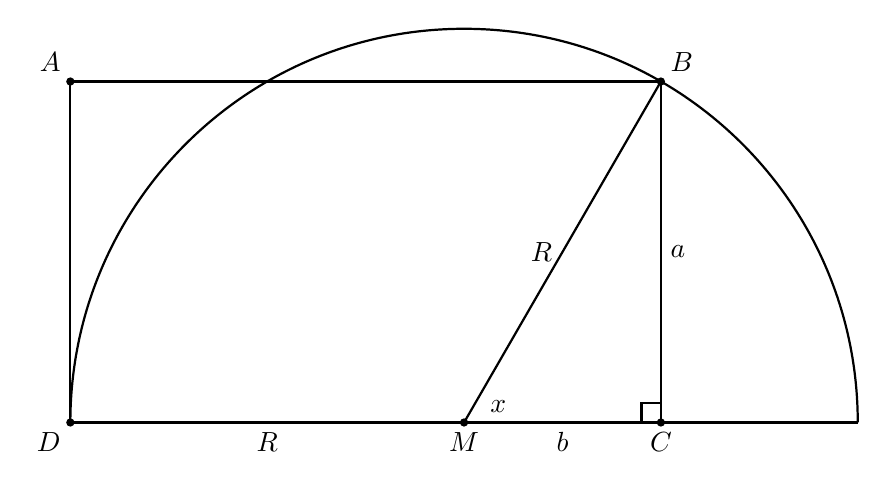
\begin{tikzpicture}%[scale=.85]
\coordinate (M) at (0,0);
\coordinate (D) at (-5,0);
\coordinate (B) at (60:5);
\coordinate (A) at (D |- B);
\coordinate (C) at (B |- M);
\draw[thick] (D) arc[start angle=180,end angle=0,radius=5cm];
\draw[thick] (D) -- (A) -- (B) -- (C);
\draw[thick] (-5,0) -- (5,0);
\draw[thick] (M) -- node[left] {$R$} (B);
\fill (A) circle(1.5pt) node[above left] {$A$};
\fill (B) circle(1.5pt) node[above right] {$B$};
\fill (C) circle(1.5pt) node[below] {$C$};
\fill (D) circle(1.5pt) node[below left] {$D$};
\fill (M) circle(1.5pt) node[below] {$M$} node[above right,xshift=6pt] {$x$};
\draw[thick,rotate=90] (C) rectangle +(7pt,7pt);
\path (D) -- node[below] {$R$} (M);
\path (M) -- node[below] {$b$} (C);
\path (C) -- node[right] {$a$} (B);
\end{tikzpicture}
\end{center}

\textbf{סעיף א}

עם הסימונים בתרשים:
\[
S(x)=a(R+b)=R\sin x(R+R\cos x)=R^2\sin x (1+\cos x)\,.
\]
נחשב את הנגזרת:
\erh{2pt}
\begin{equationarray*}{rcl}
S'(x)&=&R^2 (\cos x(1+\cos x) + \sin x \cdot -\sin x)\\
&=&R^2(\cos x + \cos^2 x -\sin^2 x)\\
&=&R^2(\cos x + \cos^2 x -(1-\cos^2 x))\\
&=&R^2(2\cos^2 x+\cos x -1 )=0\\
&=&R^2(2\cos x -1)(\cos x + 1)=0\,.
\end{equationarray*}

\np

אנחנו פוסלים את הפתרון
$\cos x=-1$
כי
$x=180$
לא יכול להיות זווית במשולש.

לכן,
$\cos x=\frac{1}{2}$, $x=60^\circ$.

הנגזרת השנייה היא:
$(2\cos^2 x+ \cos x -1)'=-4\cos x\sin x +1$.
\[
-4\cos 60\sin 60 +1=-4\cdot\frac{1}{2}\cdot\frac{\sqrt{3}}{2}+1=-\sqrt{3}+1<0\,,
\]
ןלכן נקודת הקיצון היא מקסימום.

\bigskip

\textbf{סעיף ב}

\[
\int_0^{\frac{\pi}{2}} R^2\sin x (1+\cos x) dx = \left. R^2 \cdot -\frac{1}{2}(1+\cos x)^2\right|_0^{\frac{\pi}{2}}=-\frac{R^2}{2}(1^2-2^2)=\frac{3R^2}{2}\,.
\]

\np


%%%%%%%%%%%%%%%%%%%%%%%%%%%%%%%%%%%%%%%%%%%%%%%%%%%%%%%%%%%%%%%%%%%%%%

\section{קיץ תשע"ד מועד א}

\begin{center}
\selectlanguage{english}
\includegraphics[width=\textwidth]{summer-2014a-8}
\end{center}

\vspace{-2ex}

\textbf{סעיף א}

כאשר 
$x$
עולה בערכים חיוביים, הנגזרת עולה בצורה תלולה מערכים שליליים ובצורה מתונה לערכים 
חיוביים, ולכן הפונקציה יורדת בצורה תלולה ואח"כ עולה בצורה מתונה.

כאשר 
$x$
עולה בערכים שליליים, הנגזרת יורדת בצורה מתונה מערכים חיוביים ובצורה תלולה לערכים שליליים, ולכן הפונקציה עולה בצורה מתונה ואח"כ יורדת בצורה תלולה.

לפי המידע הנתון על 
$f(x)$,
בנקודה 
$x=-1$
יש נקודה קיצון עם ערך 
$-2$
שהיא מקסימום כי השיפוע יורד ולכן הנגזרת השנייה שלילית.

בנקודה 
$x=1$
יש נקודת קיצון עם ערך
$2$
שהיא מינימום כי השיפוע עולה ולכן הנגזרת השנייה חיובית.

\begin{center}
\selectlanguage{english}
\begin{tikzpicture}%[scale=.8]
\begin{axis}[
    axis lines=center,
    xmin = -3,
    xmax = 3,
    ymin = -4,
    ymax = 4,
    yticklabel style={anchor=north east,},
]
\addplot [
    domain=-3:-.2,
    samples=50,
]
{x+(1/x)};
\addplot [
    domain=.2:3,
    samples=50,
]
{x+(1/x)};
\draw[dashed,thick] (axis cs:-3,-2) -- (axis cs:3,-2);
\draw[dashed,thick] (axis cs:-3,2) -- (axis cs:3,2);
\fill (axis cs:-1,-2) circle(1.5pt);
\fill (axis cs:1,2) circle(1.5pt);
\end{axis}
\end{tikzpicture}
\end{center}

\np

\textbf{סעיף ב}

לפי הגרף
$f'(1)=f'(-1)=0$
ונתון 
$a\neq 0$,
ולכן
$\disfrac{a-b}{a}=0$,
ו-%
$a=b$.

שוב בגלל ש-%
$a\neq 0$
אפשר לצמצם את הפרמטרים:
\[
f'(x)=\frac{a(x^2-1)}{ax^2}=\frac{x^2-1}{x^2}\,.
\]
נחשב את האיטרגל של הנגזרת כדי למצוא את הפונקציה:
\[
f(x)=\int f'(x) dx = \int \left(1-\frac{1}{x^2}\right)dx = x+\frac{1}{x}+c\,.
\]
הנגזרת מתאפסת ב-%
$\pm 1$,
ולכן נקודות המינימום והמקסימום גם הן ב-%
$\pm 1$:
\erh{10pt}
\begin{equationarray*}{rcl}
1+\frac{1}{1}+c&=&2\\
-1+\frac{1}{-1}+c&=&-2\,,
\end{equationarray*}
ולכן
$c=0$.

הפונקציה היא
$f(x)=x+\disfrac{1}{x}$.
\np


%%%%%%%%%%%%%%%%%%%%%%%%%%%%%%%%%%%%%%%%%%%%%%%%%%%%%%%%%%%%%%%%%%%%%%

\section{חורף תשע"ד}

\begin{center}
\selectlanguage{english}
\includegraphics[width=\textwidth]{winter-2014-9}
\end{center}

\vspace{-2ex}

\textbf{בבחינה זו היו שלוש שאלות בפרק השני לכן מספר השאלה הוא 
$9$
ולא 
$8$.}

\begin{center}
\selectlanguage{english}
\begin{tikzpicture}[scale=.8]
\begin{axis}[
    axis lines=center,
    xmin = 0,
    xmax = 1.5,
    ymin = 0,
    ymax = 1.5,
    ymajorticks=false,
]
\addplot [
    smooth,
    very thick,
] plot coordinates
{(1.1,1.19) (1.2,1.28) (1.3,1.36) (1.4,1.43)};
\fill (axis cs:1,0) circle(1.5pt);
\fill (axis cs:3,3) circle(1.5pt);
\end{axis}
\end{tikzpicture}
\end{center}

\textbf{סעיף א}

לפי הטבלה הפונקציה עולה מ-%
$x=1.1$
דרך 
$x=1.2$
ל-%
$x=1.3$.
נתון שאין נקודות קיצון פנימיות ולכן הנגזרת הרשאונה חיובית.

\textbf{סעיף ב}

הנגזרת השנייה שלילית כך שהנגזרת הראשונה יורדת בתחום ולכן הטענה נכונה.

\np

\textbf{סעיף ג}

\[
g'(x)=\frac{1}{2} f(x)^{-\frac{1}{2}} f'(x)\,.
\]
מסעיף א, גם 
$f(x)$
וגם
$f'(x)$
חיוביים בתחום, ולכן 
$g'(x)$
חיובי, ו-%
$g(x)$
עולה.

\textbf{סעיף ד}

\erh{12pt}
\begin{equationarray*}{rcl}
g'(x) &=& f'(x)\\
\frac{1}{2\sqrt{f(x)}} f'(x) &=& f'(x)\\
f(x)&=&\frac{1}{4}\,.
\end{equationarray*}
מצאנו שהנגזרת הראשונה חיובית כך שאפשר לצמצם אותה. לפי הטבלה,
$f(x)$
איננה פונקציה קבועה בכל התחום, לכן לא ייתכן ש-%
$g'(x) = f'(x)$.

\selectlanguage{english}

